\chapter {Contesto di riferimento}
\label{chap:contesto}

\section{Tematiche e contesto museale}
\label{sec:contesto_museale}

\subsection{Pre-Cinema}
\label{sec:precinema}

Il Cinema è un media di comunicazione di grandissimo impatto. È da lungo tempo un’arte che attira un grande numero di appassionati e di esperti. È soggetto di studi, di analisi e di approfondimenti.
Purtroppo però, le ricerche che hanno portato alla nascita del Cinema sono per lo più sconosciute al pubblico. 
Con il termine \textit{pre-cinema} si fa quindi riferimento a tutti quegli studi e tecnologie antecedenti la nascita del Cinema, datata 28 Dicembre 1895, con la prima proiezione ufficiale dei fratelli Lumière.

L’idea di sfruttare la tematica del pre-cinema per il progetto sviluppato nasce quindi dalla convinzione di poter generare curiosità riguardo una tematica non molto nota, ma verso cui esiste una base di conoscenza radicata.
Secondo Wikipedia \cite{precinema_wikipedia} “col termine pre-cinema si intendono tutti quegli esperimenti e intrattenimenti legati alla proiezione di immagini ed al movimento illusorio databili dall’antichità fino alla prima proiezione pubblica di cinematografo, organizzata dai fratelli Lumière il 28 Dicembre 1895”. 

Si parla quindi di proiezioni e dispositivi ottici, che nascono come semplici studi, per poi essere portati ad essere spettacoli per vasti pubblici. Gli spettatori erano affascinati dalle immagini e dalle esperienze che stavano vivendo, da arrivare a considerare magici gli strumenti e le tecnologie che le producevano.
Di seguito vengono analizzate alcune tecnologie e spettacoli che si sono rivelati interessanti per lo sviluppo del nostro prototipo, molte informazioni riportate sono state tratte dal libro “Quando il cinema non c’era” di Donata Pesenti Campagnoni \cite{quando_il_cinema_non_cera}:

\begin{itemize}
	\item \textbf{Camera Oscura.}
	\label{contesto_camera_oscura}
	È un dispositivo ottico basato su una scatola con un piccolo foro su di una faccia ed un piano di proiezione dell’immagine sulla faccia opposta. La luce, entrando dal foro, proietta sulla faccia opposta della scatola l’immagine capovolta di quello che si trova di fronte al foro.
	
	Il fenomeno empirico della Camera Oscura è in realtà noto sin dall’antichità, riferimenti si possono trovare già in autori come Euclide e Aristotele.
	Per molto tempo è utilizzata per osservare eclissi solari, e solo dal ‘400 in poi se ne sottolinea il potere di riprodurre immagini di ciò che ci circonda. “Leonardo da Vinci mette in luce l’analogia tra camera oscura ed occhio umano […] e da lì in poi il processo fisiologico della visione verrà spiegato sempre più spesso facendo ricorso a questo particolare fenomeno empirico a tal punto da farlo diventare, nel corso del Seicento e del Settecento, il modello più utilizzato nel campo dell’ottica fisica, la metafora per definizione dell’occhio e del suo funzionamento.
	
	\begin{figure}%[h]
		\centering
		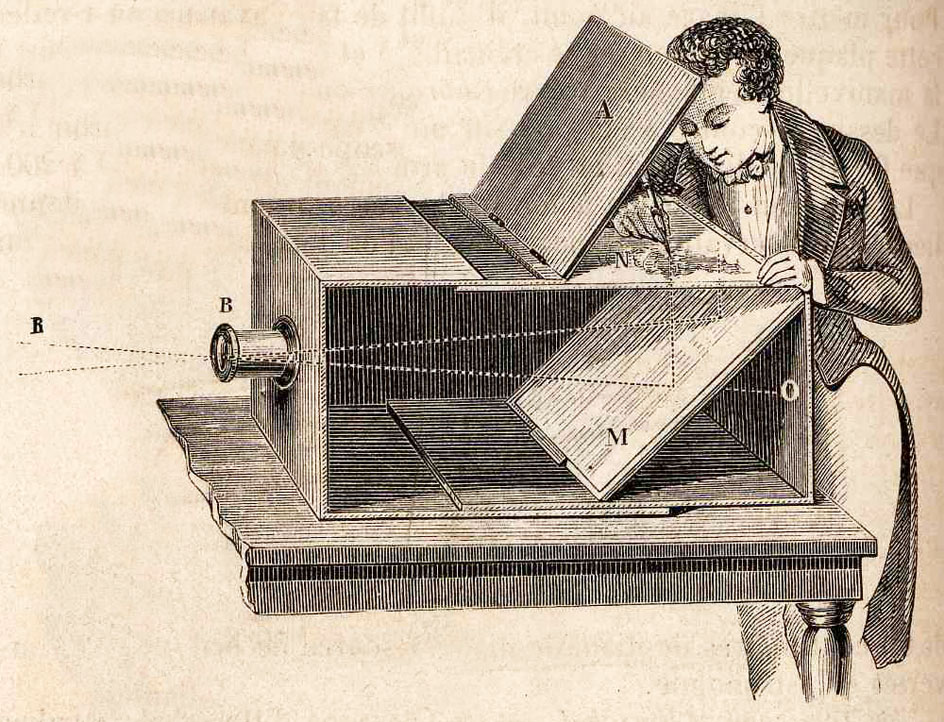
\includegraphics[width= 0.7\columnwidth]{images/contestoRiferimento/01_cameraOscura.jpg}
		\caption{Immagine della Camera Oscura.}
		\label{fig:contesto_riferimento_camera_oscura}
	\end{figure}
	
	Parallelamente, si intuiscono le possibili applicazioni del fenomeno in ambito artistico: diventa così oggetto di studio in tutto il filone di ricerca sulla prospettiva pittorica.”
	Nel Seicento fu creato un modello portatile di camera oscura, definita \textit{reflex}, In Figura~\ref{contesto_camera_oscura} ne viene mostrato il funzionamento. Prevedeva l’utilizzo di uno specchio inclinato che rifletteva l’immagine su una superficie di vetro sulla quale era possibile disegnare. Naturalmente l’utilizzo di questo strumento divenne ben presto una consuetudine nella pratica pittorica poiché consentiva all’artista di disegnare la realtà così come appariva sul vetro e in seguito rappresentò un fondamentale riferimento per tutti gli apparecchi fotografici.
	
	\item \textbf{Lanterna Magica.}
	\label{contesto_lanterna_magica}
	Antenata del moderno proiettore cinematografico, la Lanterna Magica è un apparecchio dotato di un sistema ottico e di una fonte di luce che proietta, ingrandite su uno schermo o su una parete bianca, immagini raffigurate su vetro.
	
	Il sistema ottico prevede un riflettore, un condensatore e un obiettivo: il riflettore, uno specchio concavo posizionato dietro la fonte di luce, raccoglieva i raggi luminosi e li direzionava verso il condensatore, un sistema di lenti che aveva la funzione di convergere i raggi sull’immagine dipinta e rinviarli all’obiettivo che infine proiettava l’immagine ingrandita sullo schermo.
	Il riflettore, la sorgente luminosa e il condensatore erano collocati all’interno della macchina, una semplice scatola con un camino per la fuoriuscita del fumo prodotto dalla fonte di luce; l’obiettivo era invece collocato all’esterno, sulla parte anteriore della lanterna e consentiva l’inserimento di lastre di vetro dipinte.
	In Figura~\ref{contesto_lanterna_magica} si può osservare la Lanterna Magica ed uno schema del suo funzionamento.
	
		\begin{figure}%[h]
			\centering
			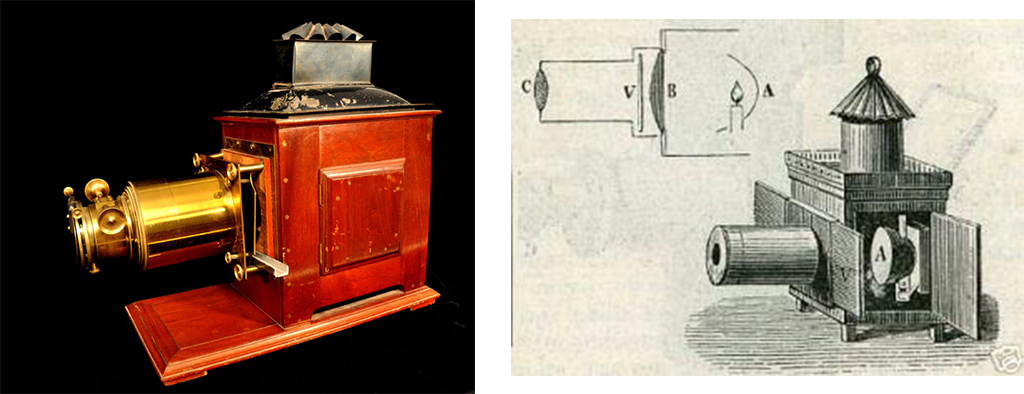
\includegraphics[width= 0.8\columnwidth]{images/contestoRiferimento/02_lanterna.jpg}
			\caption{Immagine della Lanterna Magica e schema di funzionamento.}
			\label{fig:contesto_riferimento_lanterna_magica}
		\end{figure}
	
	Nata nel Seicento barocco, la Lanterna Magica si diffuse in brevissimo tempo in ambiti e paesi diversi connotandosi come una macchina da spettacolo al momento stesso della sua comparsa. Pur nascendo come dispositivo fondato su precise leggi scientifiche, la nuova invenzione finì ben presto per apparire magica e sovrannaturale agli occhi del popolo, poiché capace di suscitare stupore, meraviglia ed emozioni profonde negli spettatori, soprattutto i meno istruiti. Per la prima volta era possibile osservare immagini a colori e in movimento che comparivano dal nulla con un effetto prodigioso, a tal punto che spesso il pubblico aveva la sensazione di poter “toccare con mano” quelle immagini favolose. Immagini che potevano apparire addirittura miracolose per gli spettatori che le osservavano senza capire il meccanismo. Non dimentichiamo che all’epoca nessuno aveva mai assistito prima ad uno spettacolo simile poiché nessuna forma di rappresentazione preesistente (come quadri, statue e affreschi) era in grado di simulare la vita e il suo movimento.
	
	Nel corso dei secoli la Lanterna venne utilizzata nei modi più diversi, non soltanto come strumento spettacolare ma anche come efficace mezzo educativo. Nel ‘600, ad esempio, il padre gesuita Kircher sfruttò le qualità prodigiose della Lanterna Magica finalizzandole all’educazione e cristianizzazione degli spettatori adoperandola come efficace strumento di evangelizzazione comprensibile a tutti, con una forza di persuasione e una potenza visiva senza precedenti. Nell’800 venne inoltre utilizzata anche in ambito scientifico e come efficace strumento per divertire istruendo e istruire divertendo. Sfruttando, ad esempio, la sua capacità di ingrandire le immagini al punto di proiettare una mosca grande come un elefante, la lanterna magica venne trasformata in un vero e proprio microscopio.
	
	\item \textbf{Dissolving Views.}
	\label{contesto_dissolving_views}
	Tra i vari utilizzi spettacolari legati alla Lanterna Magica vennero studiate raffinate tecniche di proiezione come gli incredibili effetti di dissolvenza. La nuova tecnica si basava sull’uso combinato di due o più lanterne affiancate che proiettavano, sul medesimo punto dello schermo, la graduale apparizione di un’immagine sovrapposta a quella precedente che, a poco a poco, scompariva. Spesso i soggetti proposti erano complementari riuscendo così a mostrare ad esempio il passaggio delle stagioni su un medesimo paesaggio dipinto. Vennero inoltre utilizzati particolari otturatori, diffusi in modelli diversi che consentivano di coprire gradualmente l’obbiettivo della prima lanterna e, contemporaneamente, di scoprire quello della seconda. Grazie a questo gioco di alternanza, i soggetti si \textit{dissolvevano} uno nell’altro.
	
\end{itemize}

\subsection{Situazione museale}
\label{sec:situazione_museale}

Il contesto museale ed il pubblico, che usufruisce del servizio fornito dai musei italiani, stanno pesantemente cambiando negli ultimi decenni.
L’indagine “Il museo in ascolto. Nuove strategie di comunicazione per i musei statali”, svolta da Ludovico Solima presentata nel Giugno del 2012 all’Istituto Nazionale per la Grafica di Roma \cite{MuseoInAscolto}, mostra il triplicarsi di presenze di anziani ed il dimezzamento del numero di ragazzi che si avvicinano alle strutture museali.
Il lavoro di Solima è stato svolto tra il Dicembre del 2010 e Giugno 2011 con più di 4500 questionari distribuiti in 12 musei statali italiani.

Secondo Solima, il pubblico chiede una maggiore partecipazione e non vuole più essere esclusivamente fruitore di contenuti. Con lo sviluppo di internet è pesantemente cambiato anche il paradigma di comunicazione. Attualmente il contatto tra il pubblico giovane e la struttura museale avviene principalmente in rete, e solo in maniera secondaria in forma cartacea e tramite passa parola.
La ricerca evidenzia che il 46\% del pubblico giovane effettua la visita con i propri genitori e solo il 17\% da solo. “Molto importante è l'esigenza di una \textit{visione d'insieme} che il museo dovrebbe contribuire a fornire, rispetto alla specificità dell'opera. Ciò implica il passaggio da una lettura del museo di tipo enciclopedico, ad una di tipo narrativo, attraverso una nuova strategia comunicativa che si basi più sul racconto e meno sul dato.”

Negli ultimi anni, in Italia, sono stati presi numerosi provvedimenti in direzione di un avvicinamento del pubblico più giovane al contesto museale, come l’entrata gratuita per gli Under-18 o l’apertura di alcuni musei durante le ore notturne. Ciò che emerge dai dati è comunque un'evidente mancanza di interesse nei confronti dei musei, dovuta anche alla diffusione dell’informazione su media differenti, che incentivano il pubblico ad avvicinarsi in maniera ridotta a luoghi culturali tradizionali, musei, parchi archeologici e complessi monumentali.

Secondo i dati Istat dell'annuario statistico italiano 2013 \cite{DatiIstatMusei} il 42,2\% dei giovani di età compresa tra gli 11 ed i 14 anni ed il 33\% di quelli tra i 15 e 17 anni ha visitato almeno un museo durante l’anno 2013. Sono dati che possono essere letti in maniera preoccupante soprattutto se si considera il fatto che la maggior parte delle entrate registrate sono state fatte tramite visite scolastiche. Le iniziative, in ambito didattico, permettono ai giovani di avvicinarsi ai musei ed ai luoghi culturali, ma difficilmente aumentano l’interesse dei giovani nei confronti dei beni culturali che visitano.  

\section{Contesto aziendale}
\label{sec:contesto_aziendale}

\subsection{Azienda}
\label{sec:azienda}

e-Mentor nasce nel 2004 a Torino per iniziativa dell’Ing. Manuela Martini, caratterizzandosi sin dal principio per l’attenzione alla ricerca e all’innovazione tecnologica, come attestato dai premi \textit{“Galileo Ferraris”} e \textit{“e-Content Award of Italy”}. 

Durante questi 10 anni, e-Mentor si è distinta come leader nel campo di soluzioni innovative per istituzioni, organizzazioni e aziende in ambito \textit{e-learning}, \textit{web \& mobile design}, \textit{edutainment} e \textit{software engineering}.

Nell’ambito del \textit{Mobile Design}, e-Mentor progetta e realizza applicazioni ad alta interattività per smartphone e tablet, fruibili su piattaforme iOS, Android e Windows. Attraverso l’impiego delle più aggiornate tecnologie mobili, vengono sfruttate le potenzialità del mobile computing per progettare soluzioni innovative, che spaziano dal \textit{learning on the move} - per offrire contenuti e servizi formativi interattivi in modo sempre più mirato e versatile, al \textit{situated content} - creando percorsi didattici basati sull'esplorazione del territorio con contenuti localizzati e specifici, sino agli \textit{advergames} – ideando giochi e applicativi collegati a brand ed iniziative di marketing, oppure a scopo didattico-educativo.

Grazie all'esperienza maturata nel \textit{media \& interaction design}, il team di e-Mentor progetta e sviluppa soluzioni \textit{Game-Based Learning}, quali \textit{serious games} e simulazioni interattive per facilitare l'utente nella rapida acquisizione di competenze tecniche, relazionali e organizzative attraverso il paradigma apprendimento-gioco.

Inoltre, relativamente all’ambito \textit{Web} e \textit{Software Engineering}, e-Mentor propone soluzioni web-based e stand-alone personalizzate, realizzate con tecnologie quali Php, Mysql, Java, J2ME, Ajax, in settori di applicazione come il retail, l’health care, la didattica e per ogni possibile utilizzo custom per il settore privato e pubblico.

\subsection{Situazione del progetto precedente al nostro inserimento}
\label{sec:azienda_precedente}

Il Museo del Cinema di Torino, da tempo pone l’attenzione al problema della poca affluenza di ragazzi in età adolescenziale, cercando soluzioni originali che possano invertire questa tendenza (Capitolo \ref{sec:contesto_museale}).

La collaborazione tra e-Mentor e Museo del Cinema nasce, nel 2013, per provare a porre rimedio a questo problema.
Tra le prime soluzioni proposte c’è quella di sviluppare un videogioco che avvicini i ragazzi a tematiche trattate all’interno del Museo. In seguito a mesi di lavoro e riunioni tra esperti dell’ambito \textit{learning}, artistico e del videogame, viene prodotto un documento di Design, che contiene idee di meccaniche, ambientazioni e scenari di gioco. Le tematiche che si è deciso di trattare sono quelle del \textit{pre-Cinema}, caratterizzato da tecnologie, oggettistica e curiosità per lo più ignoti al pubblico.
Il documento di Design viene presentato al bando \textit{Creative Europe, MEDIA Sub-programme, Support for Concept and Project Development of Video Games}, del Marzo 2014 \cite{CreativeEurope}.
L’idea di Design viene accolta positivamente, ma la domanda viene scartata perché il progetto viene considerato poco definito, con alcuni elementi di \textit{gameplay} non adatti ad essere finanziati e quindi lanciati sul mercato.

\subsection{Inserimento in azienda}
\label{sec:azienda_inserimento}

I nostri primi contatti con e-Mentor sono avvenuti tra Novembre e Dicembre 2014. Durante i primi incontri ci si è dedicati soprattutto all'analisi del progetto \textit{The Magic Lantern}, allo studio del contesto ed alla comprensione delle possibilità di re-design del lavoro precedentemente svolto.
Si è poi proseguito con la creazione di una timeline dettagliata di tutte le fasi di lavoro, si può far riferimento al Capitolo~\ref{sec:dev_fasi_sviluppo} per ulteriori dettagli a riguardo.
e-Mentor si è quindi fatta carico di fornirci documentazione e strumenti adeguati all'analisi del contesto, in modo da poter affrontare ogni fase del lavoro in maniera preparata ed efficiente.
Durante lo sviluppo del progetto abbiamo organizzato dei meeting periodici, ogni 3-4 settimane, con l'azienda ed esperti del settore, per ottenere linee guida sul proseguimento del lavoro, oltre che utili consigli soggettivi.
